\documentclass[a4paper,11pt]{article}
\usepackage[utf8]{inputenc}
\usepackage[italian]{babel}
\usepackage{hyperref, graphicx, float, amssymb, multirow, listings, mathtools}
\usepackage[table]{xcolor}

\graphicspath{ {./images/} }

\hypersetup{
    colorlinks=true,
    linkcolor=black,
    filecolor=magenta,
    urlcolor=cyan,
}

\title{Advanced Encryption Standard\\(AES)}
\author{Salvi Niccolò}
\date{\today}

\begin{document}
\maketitle
\tableofcontents
\newpage

\section{Introduzione}
AES\footnote{\textbf{A}dvanced \textbf{E}ncryption \textbf{S}tandard} o \textit{Rijndael} è un algoritmo di cifratura a blocchi utilizzato come standard dal governo degli USA.

Nel 1997 il NIST\footnote{\textbf{N}ational \textbf{I}nstitute of \textbf{S}tandards and \textbf{T}echnology} richiese pubblicamente proposte di algoritmi, tra i quali scegliere il sostituto del DES\footnote{\textbf{D}ata \textbf{E}ncryption \textbf{S}tandard}.

Il nuovo standard avrebbe dovuto consentire l'utilizzo di chiavi di 128, 192, 256 bit ed operare su blocchi di 128 bit in input.

Trascorso il periodo di analisi e confronto con altre proposte, nel 2002 diventa un effettivo standard.

L'algoritmo di cifratura \textit{Rijndael} è stato progettato da Joan Daemen e Vincent Rijmen ed è un'evoluzione dell'algoritmo \textit{Square} già esistente.

\subsection{Criteri di valutazione}
Il NIST utilizzò due diversi metri di giudizio nelle due fasi di valutazione degli algoritmi.

La prima valutazione si basò sulla verifica dei requisiti fondamentali:
\begin{itemize}
    \item Sicurezza:
    \begin{itemize}
        \item \textbf{Effettiva sicurezza}: da confrontare con gli altri algoritmi presenti
        \item \textbf{Casualità}: il livello di indistinguibilità dell'output dell'algoritmo da un blocco, generato in modo casuale
        \item \textbf{Solidità}: delle basi matematiche su cui si fonda l'algoritmo 
    \end{itemize}
    Siccome la dimensione minima della chiave era di 128 bit, gli attacchi a forza bruta con le tecnologie del tempo erano considerati impraticabili e per questo motivi era preferibile concentrarsi sull'analisi della resistenza dell'algoritmo rispetto agli altri attacchi noti.
    \item Costo: 
    \begin{itemize}
        \item \textbf{Requisiti di proprietà intellettuale}: l'algoritmo doveva essere accessibile e disponibile globalmente in modo gratuito
        \item \textbf{Efficienza computazionale}: valutata prima l'implementazione software, poi la velocità dell'algoritmo
        \item \textbf{Requisiti di memoria}: la memoria necessaria per l'esecuzione dell'algoritmo esaminato
    \end{itemize}
    \item Altre caratteristiche
    \begin{itemize}
        \item \textbf{Flessibilità}: preferiti gli algoritmi che rispondevano ad un numero maggiore di utenti
        \item \textbf{Fattibilità hardware e software}: l'algoritmo non doveva essere restrittivo rispetto alla piattaforma hardware o software
        \item \textbf{Semplicità}: semplicità del progetto
    \end{itemize}
\end{itemize}

Utilizzando questi criteri, gli algoritmi candidati vennero ridotti da 21 a 15 e poi 5.

I criteri utilizzati per la selezione finale:
\begin{itemize}
    \item \textbf{Ambienti con spazio limitato}: valutata la memoria richiesta per il codice, la rappresentazione di \textit{S-box} e sottochiavi
    \item \textbf{Implementazione hardware}
    \item \textbf{Crittografia e decrittografia}: se gli algoritmi sono differenti, richiedono ulteriore spazio; vi possono essere differenze nel tempo di esecuzione fra la cifratura e la decifratura
    \item \textbf{Agilità della chiave}: capacità di cambiare rapidamente la chiave, utilizzando la minima quantità possibile di risorse.
    \item \textbf{Flessibilità dei parametri}: il supporto di chiavi e blocchi di altre dimensioni e la possibilità di aumentare il numero di \textit{round}
    \item \textbf{Potenzialità sfruttamento del parallelismo}: capacità di sfruttare le funzionalità di esecuzione parallela nei processi attuali e futuri 
\end{itemize}

\subsection{Valutazione \textit{Rijndael}}
I motivi per cui l'algoritmo di \textit{Rijndael} è stato scelto sono i seguenti:
\begin{itemize}
    \item \textbf{Sicurezza generale}: non esiste alcun attacco noto in grado di romperlo. \textit{Rijndael} usa delle \textit{S-box} come componenti non lineari che dovrebbero fornire un margine di sicurezza adeguato, ma ha ricevuto qualche critica per la semplicità della sua struttura matematica
    \item \textbf{Implementazione software}: \textit{Rijndael} svolge adeguatamente le operazioni di cifratura e di decifratura in un'ampia varietà di piattaforme. Vi è una riduzione delle prestazioni quando aumentano le dimensioni delle chiavi. L'elevato parallelismo però facilita l'utilizzo efficiente delle risorse della CPU, ottenendo ottime prestazioni software
    \item \textbf{Ambienti con spazio limitato}: \textit{Rijndael} è molto adatto ad ambienti con spazio limitato dove vengono implementate la crittografia e la decrittografia. I requisiti di memoria ROM aumentano quando la crittografia e la decrittografia sono entrambe implementate
    \item \textbf{Agilità della chiave}: \textit{Rijndael} supporta il calcolo in tempo reale delle sottochiavi di crittografia; esso richiede una sola esecuzione per generare tutte le sottochiavi prima della decrittografia con una data chiave. 
    \item \textbf{Potenzialità sfruttamento del parallelismo}: ottime potenzialità per sfruttare il parallelismo nella crittografia di un singolo blocco
\end{itemize}

\section{Descrizione Algoritmo}
\subsection{La cifratura AES}
La proposta \textit{Rijndael} definiva una cifratura in cui la dimensione della chiave era 128, 192, 256 bit e vincolava la lunghezza del blocco a 128 bit.
\bigbreak
\noindent La codifica consiste in:
\begin{itemize}
    \item[-] 10 \textit{rounds} se la chiave è 128 bit
    \item[-] 12 \textit{rounds} se la chiave è 192 bit
    \item[-] 14 \textit{rounds} se la chiave è 256 bit
\end{itemize}
e ciascuno \textit{round} è formato da 4 \textit{layers}:
\begin{enumerate}
    \item \textit{Substitute Bytes} (\textit{SubBytes})
    \item \textit{ShiftRows Transformation}
    \item \textit{MixColumns Transformation}
    \item \textit{AddRoundKey}
\end{enumerate}

L'ordine delle funzioni all'interno di ogni singolo \textit{round} è il seguente:
\begin{center}
    \textit{SubBytes} $\rightarrow$ \textit{ShiftRows} $\rightarrow$ \textit{MixColumns} $\rightarrow$ \textit{AddRoundKey}
\end{center}
Il \textit{round} finale non utilizza \textit{MixColumns} e quello preliminare, \textit{round 0}, utilizza solo \textit{AddRoundKey}.

\begin{lstlisting}[language=c, frame=single, caption={Pseudo code for Chiper}][H]
Cipher(byte in[4*Nb], byte out[4*Nb], word w[Nb*(Nr+1)])
begin
    byte state[4,Nb]
    state = in

    AddRoundKey(state, w[0, Nb-1])

    for round = 1 step 1 to Nr-1
        SubBytes(state)
        ShiftRows(state)
        MixColumns(state)
        AddRoundKey(state, w[round*Nb, (round+1)*Nb-1])
    end for
    
    SubBytes(state)
    ShiftRows(state)
    AddRoundKey(state, w[Nr*Nb, (Nr+1)*Nb-1])

    out = state
end
\end{lstlisting}
\subsubsection{Numero di \textit{round}}
Il numero di \textit{round} è determinato in modo tale da rendere impossibile un attacco di forza bruta, ossia un attacco basato sulla ricerca esaustiva della chiave.

Il numero 10 è già un margine di sicurezza, poichè per il cifrario a blocchi di 128 bit non sono possibili questi tipi di attacco già con più di 6 \textit{rounds}, per le seguenti motivazioni:
\begin{enumerate}
    \item All'algoritmo \textit{Rijndael} sono sufficienti due soli \textit{rounds} per ottenere una diffusione completa dei bytes, per il fatto che i bit di \textit{State} dipendono dai byte di \textit{State} di due \textit{rounds} precedenti a quello corrente.
    \item Attacchi di crittografia lineare e differenziale sfruttano le correlazioni tra output ed input di \textit{n round} per attaccare un cifrario di $n+1$ e $n+2$ \textit{round}.
    
    Sono stati aggiuntu ulteriori 4 \textit{rounds} ai 6 che ne avrebbero garantito la sicurezza, per raddoppiare la difficoltà dell'attacco che passa da 4 a 8 \textit{rounds}.
\end{enumerate}
\subsubsection{State}
L'input dell'algoritmo è un singolo blocco di 128 bit, rappresentato da un matrice quadrata di bytes nel \href{https://nvlpubs.nist.gov/nistpubs/FIPS/NIST.FIPS.197.pdf}{\textit{FIPS PUB 197}}\footnote{Documento che contiene le caratteristiche ufficiali dell'AES.}. 

Analogamente la chiave di 128 bit è rappresentata anch'essa come una matrice quadrata di bytes e fornita come input in un array di 44 \textit{word} a 32 bit.

Questo blocco viene copiato nell'array \textit{State} che viene modificato in ogni fase della crittografia.

\begin{figure}[H]
    \centering
    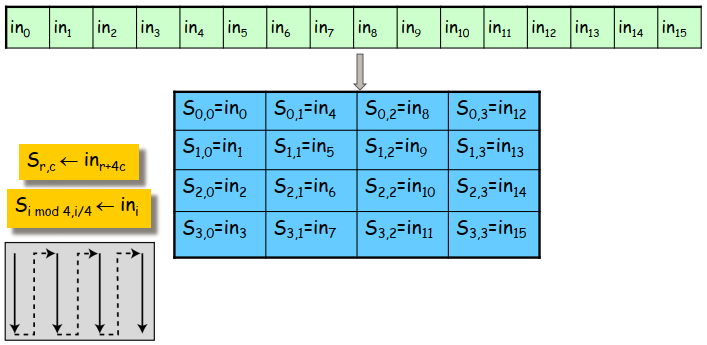
\includegraphics[scale=0.5]{stateIN}
    \caption{Input bytes $\rightarrow$ \textit{State}}
\end{figure}

Dopo la fase finale, \textit{State} viene copiato in una matrice di output.
\begin{figure}[H]
    \centering
    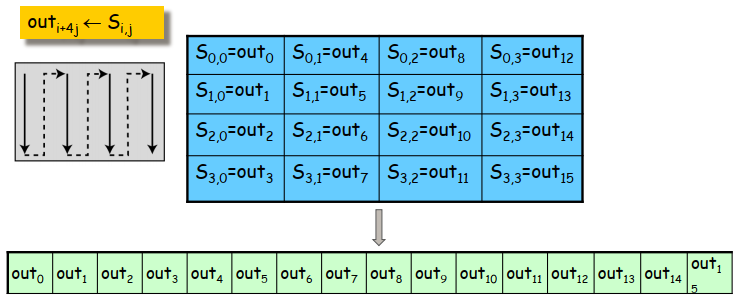
\includegraphics[scale=0.5]{stateOUT}
    \caption{\textit{States} $\rightarrow$ Output bytes}    
\end{figure}

\subsubsection{\textit{S-box}}
La \textit{S-box} viene costruita nel seguente modo:
\begin{enumerate}
    \item Inizializzare la \textit{S-box} con il valore dei byte in una sequenza ascendente riga per riga. Il valore del byte nella riga \textit{x} e colonna \textit{y} è \{xy\}.\\
    La prima riga contiene \{00\}, \{01\}, \{02\}, ..., \{0F\}\\
    La seconda riga contiene \{10\}, \{11\}, \{12\}, ..., \{1F\}
    \item Associare a ciascun byte della \textit{S-box} il suo inverso moltiplicativo nel campo finito $GF(2^8)$. \\
    \{00\} rimane \{00\}
    \item Considerare che ciascun byte della \textit{S-box} è costituito da 8 bit con \textit{($b_7$, $b_6$, $b_5$, $b_4$, $b_3$, $b_2$, $b_1$, $b_0$)}. Applicare la seguente trasformazione a ciascun bit di ciascun byte della \textit{S-box}:
    \begin{center}
        $b_i'\, = \, b_i \, \oplus \, b_{(i+4)mod8} \, \oplus \, b_{(i+5)mod8} \, \oplus \, b_{(i+6)mod8} \, \oplus \, b_{(i+7)mod8} \, \oplus \, c_i$
    \end{center}
    dove $c_i$ è l'i-esimo bit del byte \textit{c} con il valore \{63\}: 01100011.
\end{enumerate}
\begin{itemize}
    \item[] $b_0'\, = \, b_0 \, \oplus \, b_4 \, \oplus \, b_5 \, \oplus \, b_6 \, \oplus \, b_7 \, \oplus \, 0$
    \item[] $b_1'\, = \, b_1 \, \oplus \, b_5 \, \oplus \, b_6 \, \oplus \, b_7 \, \oplus \, b_0 \, \oplus \, 1$
\end{itemize}

\begin{table}[H]
    \centering
    \makebox[\textwidth]{
    \begin{tabular}{@{}|c|c|*{16}{c|}}
        \hline
        \multicolumn{1}{|c}{} &\multicolumn{17}{c|}{y}\\
        \cline{2-18}
        \multicolumn{1}{|c|}{} & & \cellcolor{gray!25}\textbf{0} & \cellcolor{gray!25}\textbf{1} & \cellcolor{gray!25}\textbf{2} & \cellcolor{gray!25}\textbf{3} & \cellcolor{gray!25}\textbf{4} & \cellcolor{gray!25}\textbf{5} & \cellcolor{gray!25}\textbf{6} & \cellcolor{gray!25}\textbf{7} & \cellcolor{gray!25}\textbf{8} & \cellcolor{gray!25}\textbf{9} & \cellcolor{gray!25}\textbf{A} & \cellcolor{gray!25}\textbf{B} & \cellcolor{gray!25}\textbf{C} & \cellcolor{gray!25}\textbf{D} & \cellcolor{gray!25}\textbf{E} & \cellcolor{gray!25}\textbf{F} \\ \cline{2-18}
        \multirow{16}*{x}
        & \cellcolor{gray!25}\textbf{0} & 63 & 7C & 77 & 7B & F2 & 6B & 6F & C5 & 30 & 01 & 67 & 2B & FE & D7 & AB & 76
        \\ \cline{2-18}
        & \cellcolor{gray!25}\textbf{1} & CA & 82 & C9 & 7D & FA & 59 & 47 & F0 & AD & D4 & A2 & AF & 9C & A4 & 72 & C0
        \\ \cline{2-18}
        & \cellcolor{gray!25}\textbf{2} & B7 & FD & 93 & 26 & 36 & 3F & F7 & CC & 34 & A5 & E5 & F1 & 71 & D8 & 31 & 15
        \\ \cline{2-18}
        & \cellcolor{gray!25}\textbf{3} & 04 & C7 & 23 & C3 & 18 & 96 & 05 & 9A & 07 & 12 & 80 & E2 & EB & 27 & B2 & 75
        \\ \cline{2-18}
        & \cellcolor{gray!25}\textbf{4} & 09 & 83 & 2C & 1A & 1B & 6E & 5A & A0 & 52 & 3B & D6 & B3 & 29 & E3 & 2F & 84
        \\ \cline{2-18}
        & \cellcolor{gray!25}\textbf{5} & 53 & D1 & 00 & ED & 20 & FC & B1 & 5B & 6A & CB & BE & 39 & 4A & 4C & 58 & CF
        \\ \cline{2-18}
        & \cellcolor{gray!25}\textbf{6} & D0 & EF & AA & FB & 43 & 4B & 33 & 85 & 45 & F9 & 02 & 7F & 50 & 3C & 9F & A8
        \\ \cline{2-18}
        & \cellcolor{gray!25}\textbf{7} & 51 & A3 & 40 & 8F & 92 & 9D & 38 & F5 & BC & B6 & DA & 21 & 10 & FF & F3 & D2
        \\ \cline{2-18}
        & \cellcolor{gray!25}\textbf{8} & CD & 0C & 13 & EC & 5F & 97 & 44 & 17 & C4 & A7 & 7E & 3D & 64 & 5D & 19 & 73
        \\ \cline{2-18}
        & \cellcolor{gray!25}\textbf{9} & 60 & 81 & 4F & DC & 22 & 2A & 90 & 88 & 46 & EE & B8 & 14 & DE & 5E & 0B & DB
        \\ \cline{2-18}
        & \cellcolor{gray!25}\textbf{A} & E0 & 32 & 3A & 0A & 49 & 06 & 24 & 5C & C2 & D3 & AC & 62 & 91 & 95 & E4 & 79
        \\ \cline{2-18}
        & \cellcolor{gray!25}\textbf{B} & E7 & C8 & 37 & 6D & 8D & D5 & 4E & A9 & 6C & 56 & F4 & EA & 65 & 7A & AE & 08
        \\ \cline{2-18}
        & \cellcolor{gray!25}\textbf{C} & BA & 78 & 25 & 2E & 1C & A6 & B4 & C6 & E8 & DD & 74 & 1F & 4B & BD & 8B & 8A
        \\ \cline{2-18}
        & \cellcolor{gray!25}\textbf{D} & 70 & 3E & B5 & 66 & 48 & 03 & F6 & 0E & 61 & 35 & 57 & B9 & 86 & C1 & 1D & 9E
        \\ \cline{2-18}
        & \cellcolor{gray!25}\textbf{E} & E1 & F8 & 98 & 11 & 69 & D9 & 8E & 94 & 9B & 1E & 87 & E9 & CE & 55 & 28 & DF
        \\ \cline{2-18}
        & \cellcolor{gray!25}\textbf{F} & 8C & A1 & 89 & 0D & BF & E6 & 42 & 68 & 41 & 99 & 2D & 0F & B0 & 54 & BB & 16\\ \cline{2-18}
        \hline
    \end{tabular}}
    \caption{\textit{S-box}}
\end{table}

Le proprietà della \textit{S-box} sono le seguenti:
\begin{itemize}
    \item L'output non è una funziona lineare dell'input: si tratta dell'unica operazione non lineare dell'intero algoritmo
    \item $InvSbox(S\-box(a)) = a \rightarrow$ invertibile
    \item $Sbox(a) \neq InvSbox(a) \rightarrow$ no self-invertibile
    \item Progettata per resistere ad attacchi crittoanalitici
\end{itemize}

\subsubsection{SubBytes}
La \textit{Trasformazione SubBytes} è una ricerca su tabella.
AES definisce una matrice di 16x16 byte chiamata \textit{S-box} che contiene una permutazione di tutti i 256 valori a 8 bit.

Ogni singolo byte di \textit{State} viene mappato in nuovo byte: i primi 4 bit indicano la riga ed i secondi 4 bit la colonna. Tali valori di riga e colonna rappresentato gli indici della \textit{S-box} per selezionare un valore univoco di output a 8 bit.
\begin{figure}[h]
    \centering
    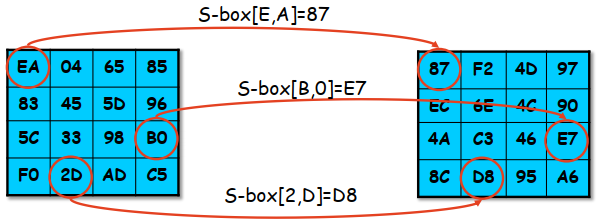
\includegraphics[scale=0.5]{subbytes}
    \caption{\textit{State} $\xrightarrow[]{\text{\textit{S-box}}}$ \textit{State'}}
\end{figure}


\subsubsection{ShiftRows}
La \textit{Trasformazione ShiftRows} consiste nello scorrimento di byte nell'array \textit{State}:
\begin{itemize}
    \item{$1^a$ riga} non viene modificata
    \item{$2^a$ riga} scorrimento circolare a sinistra di 1 byte
    \item{$3^a$ riga} scorrimento circolare a sinistra di 2 byte
    \item{$4^a$ riga} scorrimento circolare a sinistra di 3 byte
\end{itemize}

\begin{figure}[h]
    \centering
    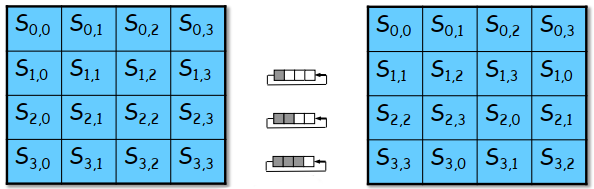
\includegraphics[scale=0.5]{shiftrows}
    \caption{ShiftRows di \textit{State}}
\end{figure}
\subsubsection{MixColumns}
La \textit{Trasformazione MixColumns} opera su ogni singola colonna. Ciascun byte di una colonna viene mappato in un nuovo valore che è una funzione dei 4 byte presenti nella colonna.
L'operazione è definita dalla seguente moltiplicazione di matrici su \textit{State}:

\begin{figure}[H]
    \centering
    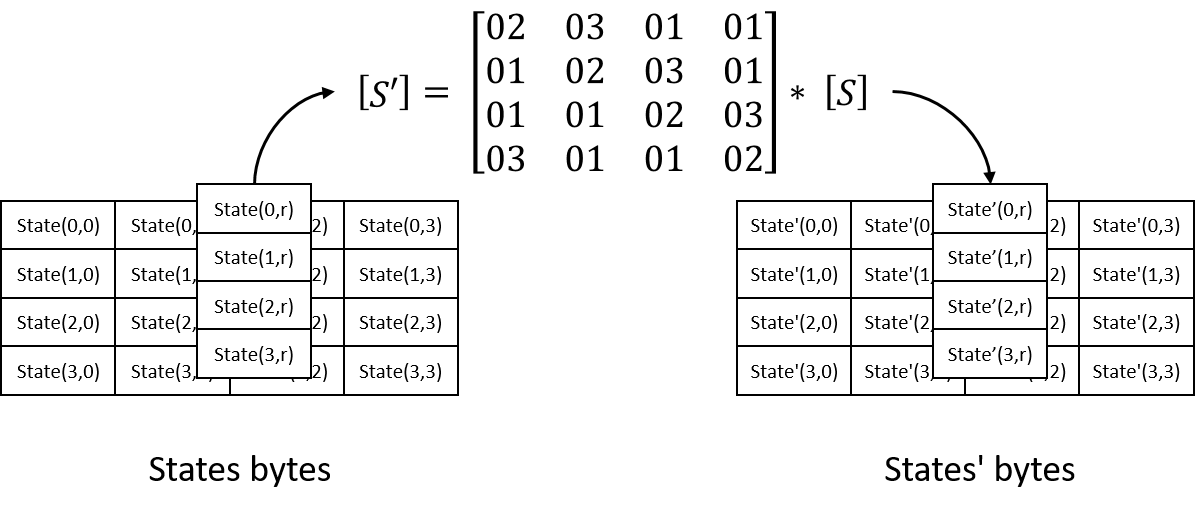
\includegraphics[scale=0.4]{mixcolumns}
    \caption{\textit{State} * Matrix = \textit{State'}}
\end{figure}
Ciascun elemento è somma dei prodotti degli elementi di una riga e una colonna.
\begin{center}
    $0 \leq j \leq 3$\bigbreak
    $s_{0, j}' = (\{02\} \cdot s_{0, j}) \oplus (\{03\} \cdot s_{1, j}) \oplus s_{2, j} \oplus s_{3, j}$\bigbreak
    $s_{1, j}' = s_{0, j} \oplus (\{02\} \cdot s_{1, j}) \oplus (\{03\} \cdot s_{2, j}) \oplus s_{3, j}$\bigbreak
    $s_{2, j}' = s_{0, j} \oplus s_{1, j} \oplus (\{02\} \cdot s_{2, j}) \oplus (\{03\} \cdot s_{3, j})$\bigbreak
    $s_{3, j}' = (\{03\} \cdot s_{0, j}) \oplus s_{1, j} \oplus s_{2, j} \oplus (\{02\} \cdot s_{3, j}) $
\end{center}
Dove $\cdot$ si utilizza per indicare la moltiplicazione sul campo finito $GF(2^8)$ e $\oplus$ per indicare l'operazione XOR bit a bit, che corrisponde alla somma in $GF(2^8)$.
\begin{center}
    \begin{tabular}{|c|c|c|c|}
        \hline
        \cellcolor{gray!25}87 & F2 & \cellcolor{gray!25}4D & 97 \\
        \hline 
        \cellcolor{gray!25}6E & 4C & \cellcolor{gray!25}90 & EC \\  
        \hline
        \cellcolor{gray!25}46 & E7 & \cellcolor{gray!25}4A & C3 \\  
        \hline
        \cellcolor{gray!25}A6 & 8C & \cellcolor{gray!25}D8 & 95 \\  
        \hline
    \end{tabular}
    $\rightarrow$
    \begin{tabular}{|c|c|c|c|}
        \hline
        \cellcolor{gray!25}47 & 40 & \cellcolor{gray!25}A3 & 4C \\
        \hline 
        \cellcolor{gray!25}37 & D4 & \cellcolor{gray!25}70 & 9F \\  
        \hline
        \cellcolor{gray!25}94 & E4 & \cellcolor{gray!25}3A & 42 \\  
        \hline
        \cellcolor{gray!25}ED & A5 & \cellcolor{gray!25}A6 & BC \\  
        \hline
    \end{tabular}
\end{center}
\begin{center}
    \begin{center}
        $s_{0, 0}' = (\{02\} \cdot \{87\}) \oplus (\{03\} \cdot \{6E\}) \oplus \{46\} \oplus \{A6\} = \{47\}$\bigbreak
        $s_{1, 0}' = \{87\} \oplus (\{02\} \cdot \{6E\}) \oplus (\{03\} \cdot \{46\}) \oplus \{A6\} = \{37\}$\bigbreak
        $s_{2, 0}' = \{87\} \oplus \{6E\} \oplus (\{02\} \cdot \{46\}) \oplus (\{03\} \cdot \{A6\}) = \{94\}$\bigbreak
        $s_{3, 0}' = (\{03\} \cdot \{87\}) \oplus \{6E\} \oplus \{46\} \oplus (\{02\} \cdot \{A6\}) = \{ED\}$
    \end{center}
\end{center}

\bigbreak
Il documento AES descrive anche un altro modo per eseguire la \textit{Trasformazione MixColumns}: ciascuna colonna di \textit{State} viene definita come polinomio di quattro termini con coefficienti in $GF(2^8)$.

Ciascuna colonna viene moltiplicata modulo $(x^4 + 1)$ per il polinomio fisso $a(x)$ dato da:
\begin{center}
    $a(x) = \{03\}x^3 + \{01\}x^2 + \{01\}x + \{02\}$
\end{center}

\subsubsection{AddRoundKey}
Nella \textit{Trasformazione AddRoundKey} viene inserita la chiave segreta che rende il cifrario sicuro (le altre trasformazioni sono note e quindi facilmente invertibili).

Nella \textit{Trasformazione AddRoundKey} i 128 bit di \textit{State} vengono sottoposti a uno XOR bit a bit con i 128 bit della \textit{Round Key}\footnote{Ad ogni \textit{round} la chiave aggiunta è diversa e ricavata ricorsivamente dalle precedenti.}: si tratta di una somma vettoriale in $\mathbb{Z}_2^{128}$ tra i 4 byte della colonna di \textit{State} ed $Nb$ della chiave schedulata.

La sicurezza è garantita dalla complessità dell'espansione della chiave di fase e dalla complessità degli altri stadi di AES.
\begin{figure}[H]
    \centering
    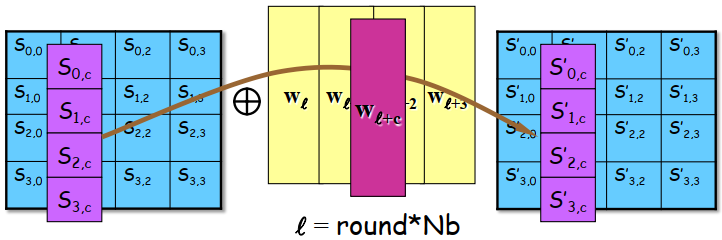
\includegraphics[scale=0.5]{addroundkey}
    \caption{\textit{AddRoundKey}}
\end{figure}

\subsubsection{Espansione chiave}
\textit{Rijndael} implementa una routine di espansione della chiave per generare una chiave schedulata, partendo da quella presa in input.

L'algoritmo di espansione della chiave genera un totale di $Nb * (Nr +1)$ \textit{words}: il processo di cifratura richiede un insieme iniziale di $Nb$ \textit{words} ed ad ogni esecuzione di un \textit{round} vengono richiesti $Nb$ \textit{words} della chiave.

La chiave schedulata risultante consiste di un array lineare di \textit{words} a 32 bit.

\begin{lstlisting}[language=c, caption={Pseudo Code for the Key Expansion}, frame=single][H]
KeyExpansion(byte key[4*Nk], word w[Nb*(Nr+1)], Nk)
begin
    word temp
    i = 0

    while (i < Nk)
        w[i] = word(key[4*i], key[4*i+1], key[4*i+2], key[4*i+3])
        i = i+1
    end while
    
    i = Nk
    while (i < Nb * (Nr+1))
        temp = w[i-1]
        if (i mod Nk = 0)
            temp = SubWord(RotWord(temp)) xor Rcon[i/Nk]
        else if (Nk > 6 and i mod Nk = 4)
            temp = SubWord(temp)
        end if
        
        w[i] = w[i-Nk] xor temp
        i = i + 1
    end while
end
\end{lstlisting}
\bigbreak
Le prime $Nk$ (rappresenta il numero di \textit{words} a 32 bit che formano la chiave di cifratura) \textit{words} della chiave espansa sono ottenute direttamente dalla chiave di cifratura presa in input.
\bigbreak
Ogni word successiva, $W[i]$, è uguale allo XOR tra la \textit{word} precedente e quella di $Nk$ posizioni più indietro.
\begin{center}
    $W[i] = W[i-1] \oplus W[i-Nk]$
\end{center}
\bigbreak
Per le \textit{words} con posizioni multiple di $Nk$, viene applicata a $W[i-1]$ una trasformazione, seguita da uno XOR con una costante di round $\textit{Rcon[i]}$ ed infine viene eseguito la XOR con la \textit{word} di $Nk$ posizioni precedenti (come definito nel punto precedente).
\bigbreak
Questa trasformazione consiste in:
\begin{description}
    \item[RotWord()] compie uno scorrimento circolare a sinistra di un byte sulla \textit{Word}
    \item[SubWord()] utilizzando la \textit{S-box} di AES sostituisce ogni byte della \textit{Word} in input 
\end{description}
\bigbreak
L'algoritmo di espansione della chiave per una chiave di 256 bit  si compota diversamente rispetto ad una chiave di 128 o 192 bit, in quanto cambia il valore di $Nk$.

\subsection{La decifratura di AES}
AES non è un cifrario di \textit{Feistel}, al contrario del precedente algoritmo DES.

Pertanto, la cifratura e la decifrazione utilizzano due algoritmi differenti.
\bigbreak
Ogni funzione della cifratura ha una sua funzione inversa:
\begin{enumerate}
    \item \textit{InvSubBytes} utilizza la permutazione inversa \textit{InvS-box}
    \item \textit{InvShiftRows} si ottiene facendo scorrere le righe a destra, invece che a sinistra.
    \item \textit{InvMixColumns} sfrutta la matrice invertita usata in \textit{MixColumns}
    \item \textit{AddRoundKey} coincide con il suo inverso
\end{enumerate}
\bigbreak\noindent
L'ordine delle funzioni all'interno di ogni singolo \textit{round} è il seguente:
\begin{center}
    \textit{InvShiftRows} $\rightarrow$ \textit{InvSubBytes} $\rightarrow$ \textit{AddRoundKey} $\rightarrow$ \textit{InvMixColumns}
\end{center}
\begin{lstlisting}[language=c, caption={Pseudo Code for the Inverse Cipher}, frame=single][H]
InvCipher(byte in[4*Nb], byte out[4*Nb], word w[Nb*(Nr+1)])
begin
    byte state[4,Nb]
    state = in

    AddRoundKey(state, w[Nr*Nb, (Nr+1)*Nb-1])
    
    for round = Nr-1 step -1 downto 1
        InvShiftRows(state)
        InvSubBytes(state)
        AddRoundKey(state, w[round*Nb, (round+1)*Nb-1])
        InvMixColumns(state)
    end for

    InvShiftRows(state)
    InvSubBytes(state)
    AddRoundKey(state, w[0, Nb-1])

    out = state
end
\end{lstlisting}

\subsubsection{\textit{InvS-box}}
La \textit{InvS-box} è un'altra tabella che implementa la permutazione inversa, calcolata nella seguente maniera:
\begin{center}
    $b_i' = b_i \oplus b_{(i+2)mod8} \oplus b_{(i+5)mod8} \oplus b_{(i+7)mod8} \oplus d_i$\bigbreak
    $d = \{05\}$
\end{center}
\begin{table}[H]
    \centering
    \makebox[\textwidth]{
    \begin{tabular}{@{}|c|c|*{16}{c|}}
        \hline
        \multicolumn{1}{|c}{} &\multicolumn{17}{c|}{y}\\
        \cline{2-18}
        \multicolumn{1}{|c|}{} & & \cellcolor{gray!25}\textbf{0} & \cellcolor{gray!25}\textbf{1} & \cellcolor{gray!25}\textbf{2} & \cellcolor{gray!25}\textbf{3} & \cellcolor{gray!25}\textbf{4} & \cellcolor{gray!25}\textbf{5} & \cellcolor{gray!25}\textbf{6} & \cellcolor{gray!25}\textbf{7} & \cellcolor{gray!25}\textbf{8} & \cellcolor{gray!25}\textbf{9} & \cellcolor{gray!25}\textbf{A} & \cellcolor{gray!25}\textbf{B} & \cellcolor{gray!25}\textbf{C} & \cellcolor{gray!25}\textbf{D} & \cellcolor{gray!25}\textbf{E} & \cellcolor{gray!25}\textbf{F} \\ \cline{2-18}
        \multirow{16}*{x}
        & \cellcolor{gray!25}\textbf{0} & 52 & 09 & 6A & D5 & 30 & 36 & A5 & 38 & DF & 40 & A3 & 9E & 81 & F3 & D7 & FB
        \\ \cline{2-18}
        & \cellcolor{gray!25}\textbf{1} & 7C & E3 & 39 & 82 & 9B & 2F & FF & 87 & 34 & 8E & 43 & 44 & C4 & DE & E9 & CB
        \\ \cline{2-18}
        & \cellcolor{gray!25}\textbf{2} & 54 & 7B & 94 & 32 & A6 & C2 & 23 & 3D & EE & 4C & 95 & 0B & 42 & FA & C3 & 4E
        \\ \cline{2-18}
        & \cellcolor{gray!25}\textbf{3} & 08 & 2E & A1 & 66 & 28 & D9 & 24 & B2 & 76 & 5B & A2 & 49 & 6D & 8B & D1 & 25
        \\ \cline{2-18}
        & \cellcolor{gray!25}\textbf{4} & 72 & F8 & F6 & 64 & 86 & 68 & 98 & 16 & D4 & A4 & 5C & CC & 5D & 65 & B6 & 92
        \\ \cline{2-18}
        & \cellcolor{gray!25}\textbf{5} & 6C & 70 & 48 & 50 & FD & ED & B9 & DA & 5E & 15 & 46 & 57 & A7 & 8D & 9D & 84
        \\ \cline{2-18}
        & \cellcolor{gray!25}\textbf{6} & 90 & D8 & AB & 00 & 8C & BC & D3 & 0A & F7 & E4 & 58 & 05 & B8 & B3 & 45 & 06
        \\ \cline{2-18}
        & \cellcolor{gray!25}\textbf{7} & D0 & 2C & 1E & 8F & CA & 3F & 0F & 02 & C1 & AF & BD & 03 & 01 & 13 & 8A & 6B
        \\ \cline{2-18}
        & \cellcolor{gray!25}\textbf{8} & 3A & 91 & 11 & 41 & 4F & 67 & DC & EA & 97 & F2 & CF & CE & F0 & B4 & E6 & 73
        \\ \cline{2-18}
        & \cellcolor{gray!25}\textbf{9} & 96 & AC & 74 & 22 & E7 & AD & 35 & 85 & E2 & F9 & 37 & E8 & 1C & 75 & DF & 6E
        \\ \cline{2-18}
        & \cellcolor{gray!25}\textbf{A} & 47 & F1 & 1A & 71 & 1D & 29 & C5 & 89 & 6F & B7 & 62 & 0E & AA & 18 & BE & 1B
        \\ \cline{2-18}
        & \cellcolor{gray!25}\textbf{B} & FC & 56 & 3E & 4B & C6 & D2 & 79 & 20 & 9A & DB & C0 & FE & 78 & CD & 5A & F4
        \\ \cline{2-18}
        & \cellcolor{gray!25}\textbf{C} & 1F & DD & A8 & 33 & 88 & 07 & C7 & 31 & B1 & 12 & 10 & 59 & 27 & 80 & EC & 5F
        \\ \cline{2-18}
        & \cellcolor{gray!25}\textbf{D} & 60 & 51 & 7F & A9 & 19 & B5 & 4A & 0D & 2D & E5 & 7A & 9F & 93 & C9 & 9C & EF
        \\ \cline{2-18}
        & \cellcolor{gray!25}\textbf{E} & A0 & E0 & 3B & 4D & AE & 2A & F5 & B0 & C8 & EB & BB & 3C & 83 & 53 & 99 & 61
        \\ \cline{2-18}
        & \cellcolor{gray!25}\textbf{F} & 17 & 2B & 04 & 7E & BA & 77 & D6 & 26 & E1 & 69 & 14 & 63 & 55 & 21 & 0C & 7D
        \\ \cline{2-18}
        \hline
    \end{tabular}}
    \caption{\textit{InvS-box}}
\end{table}

\subsubsection{InvShiftRows}
La \textit{Trasformazione InvShiftRows} applica all'array \textit{State} uno scorrimento circolare nelle righe, allo stesso modo della corrispettiva funzione di cifratura, ma nella direzione opposta: verso destra.
\begin{figure}[H]
    \centering
    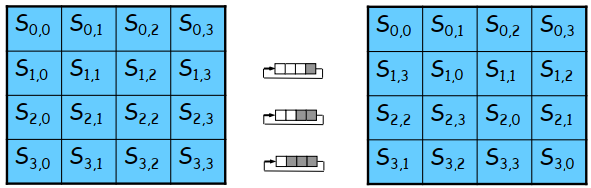
\includegraphics[scale=0.5]{invshiftrows}
    \caption{\textit{InvShiftRows}}
\end{figure}

\subsubsection{InvSubBytes}
La \textit{Trasformazione InvSubBytes} funziona esattamente allo stesso modo della sua corrispettiva diretta, cambia solo la \textit{S-box} è una tabella che implementa la permutazione inversa.

\subsubsection{InvMixColumns}
\begin{figure}[H]
    \centering
    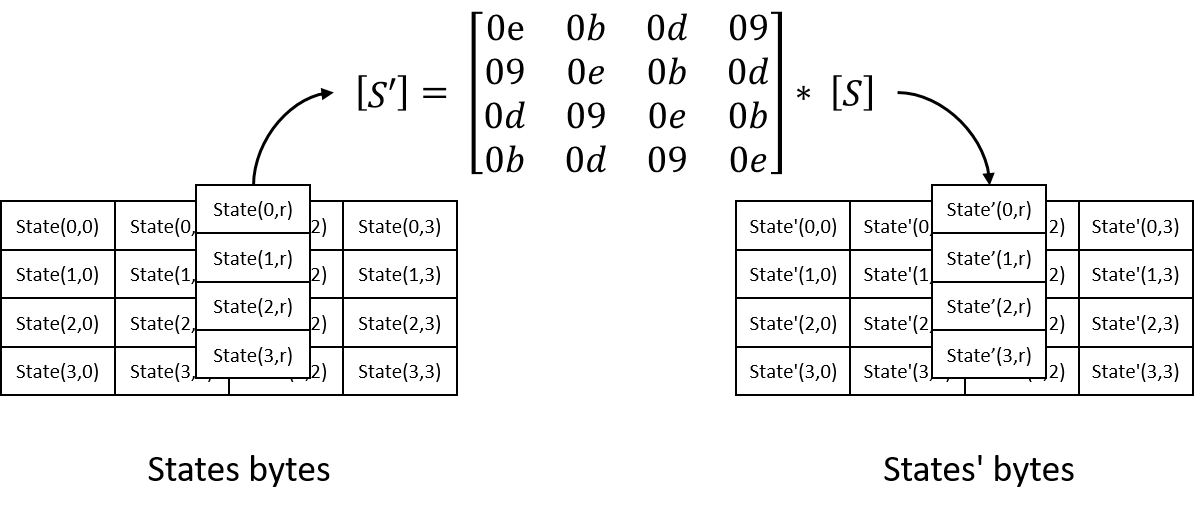
\includegraphics[scale=0.4]{invmixcolumns}
    \caption{\textit{InvMixColumns}}
\end{figure}

\subsubsection{Cifratura inversa equivalente}
Predisporre di due algoritmi differenti per le operazione di cifratura e di decifratura rappresenta uno svantaggio dal punto di vista implementativo.

E' stato implementato un algoritmo equivalente a quello di decrittografia, che utilizza sempre le funzioni inverse nel medesimo ordine del processo di cifrazione.

\begin{center}
    \textit{InvSubBytes} $\rightarrow$ \textit{InvShiftRows} $\rightarrow$ \textit{InvMixColumns} $\rightarrow$ \textit{AddRoundKey}
\end{center}
\begin{lstlisting}[language=c, caption={Pseudo Code for the Equivalent Inverse Cipher}, frame=single][H]
EqInvCipher(byte in[4*Nb], byte out[4*Nb], word dw[Nb*(Nr+1)])
begin
    byte state[4,Nb]
    state = in
    
    AddRoundKey(state, dw[Nr*Nb, (Nr+1)*Nb-1])
    for round = Nr-1 step -1 downto 1
        InvSubBytes(state)
        InvShiftRows(state)
        InvMixColumns(state)
        AddRoundKey(state, dw[round*Nb, (round+1)*Nb-1])
    end for
    
    InvSubBytes(state)
    InvShiftRows(state)
    AddRoundKey(state, dw[0, Nb-1])
    
    out = state
end
\end{lstlisting}

Rispetto all'algoritmo di decifratura precedente è necessario scambiare le prime due trasformazioni tra loro, così come le seconde due.
\paragraph{Scambio tra \textit{InvShiftRows} e \textit{InvSubBytes}} \textit{InvShiftRows} altera la sequenza dei bytes di \textit{State} ma non il suo contenuto, mentre \textit{InvSubBytes} ne altera il contenuto ma non la sequenza dei bytes. Per un determinato \textit{State} $S_i$: 
\begin{center}
    $\textit{InvShiftRows}[\textit{InvSubBytes}(S_i)] = \textit{InvSubBytes}[\textit{InvShiftRows}(S_i)]$
\end{center} 
\paragraph{Scambio tra \textit{AddRoundKey} e \textit{InvMixColumns}} Per un determinato \textit{State} $S_i$ ed una determinata chiave di fase $W_j$:
\begin{center}
    $\textit{InvMixColumns}(S_i \oplus W_j) = [\textit{InvMixColumns}(S_i)] \oplus [\textit{InvMixColumns}(W_i)]$
\end{center}

Per poter applicare lo scambio, basta applicare \textit{InvMixColumns} alla chiave di fase prima di aggiungerla allo \textit{State} corrente.
\end{document}